\section{Experimental method}

This experiment consists of four parts. First the calibration of the microscope. Secondly size measurements on respectively a human hair, an optical glass fibre and starch particles. Thirdly determining the birefringence of an unknown crystal and finally the computerized improvement of an image of a biological fungus sample. The different experimental methods will be treated separately.\\
\\
The microscope that is used in all experiments is a Leica DM EP microscope. Its manual can be found in appendix \ref{appendix_manual}. This microscope is used in combination with $4\times$, $10\times$, $40\times$ Hi Plan POL objectives with respectfully a 0.10, 0.22 and 0.65 numerical aperture. A color CCD camera in combination with NI Vision Assistant software is used to acquire digital images.

\subsection{Calibration}
\label{expmeth_calibration}
A microscopic ruler is used to measure the length that corresponds to one pixel in an image, $l_{pixel}$. This is achieved by focussing on a 1 mm, 100 division ruler and measuring the distance between two focussed, distant division lines and comparing the number of pixels to the physical length. The NI software is used to find the exact location of these two lines and subsequently find the perpendicular projection distance, $n_{pixels}$. This procedure is repeated for all three objectives. \\
\bigskip 
With the aid of a 1951 USAF resolution target, the resolving power of each objective can be found. First taking a focussed gray-scale image  on the target and then taking a perpendicular intensity profile for each well defined three-bar structure (see Figure \ref{fig:resolution_target}). This intensity profile is exported by NI Vision to a CSV file directly so we dont suffer from any compression, a file which can be easily read by a python peakfinding script ( an example of which can be seen in the next section's figure \ref{fig:linetrace}). The high and low intensity values will be used to calculate the visibility using equation \ref{eq_visibility} and the corresponding spatial frequency. This is repeated for all three objectives.\\

\begin{equation}
  V = \frac{I_{max}-I_{min}}{I_{max}+I_{min}}
  \label{eq:visibility}
\end{equation}
\subsection{Microscopic size measurements}
All microscopic size measurements are made by measuring pixels and comparing this to the corresponding pixel length. This is done for images with the $40\times$ objective since this gives the smallest error.



\subsubsection*{Human hair and optical glass fibre}

Measuring the thickness of the human hair and optical glass fibre is done with the aid of the NI Vision software. First finding the two straight lines of the outer edges and subsequently measuring the perpendicular distance between the two, $n_{hair}$ and $n_{gf}$ in pixels. The physical size, $d_{hair}$ and $d_{gf}$, and error can be calculated using respectfully equation \ref{eq_distance} and \ref{eq_u_distance}. 


\subsubsection*{Starch particles}

In order to measure the size of individual starch particles, a small amount of starch is mixed with oil and images are taken at different locations in the mixture. For ellipse-shaped particles that are focussed in the image, an ellipse can manually be fitted. Using the values for the major and minor axis, respectfully $a$ and $b$, the estimated errors and equations \ref{eq_ellipse} and \ref{eq_u_ellipse}, the area of the ellipse, $A$, and corresponding error can be calculated.\\
For this experiment it was chosen to find the ellipse size for 30 particles.


\subsection{Birefringence}

In order to find the birefringence, $\Delta n$, of the unknown crystal, it is placed in the microscope with the polariser crossed with respect to the analyser. The crystal is then turned until bright colours can be seen. Now the difference in path length, $\Delta l_{path}$, is measured as a function of the thickness, $D$, of the crystal. $D$ can be found by viewing a border between adjacent colour planes and subsequently noting the focussing position, $f$, of each colour plane. Taking the difference between two values of $f$ will give the difference in thickness, $\Delta d$, between two colour planes. Simple addition and subtraction will give the values for $D$. The bottom of the sample (black) is also to be taken into account with the same procedure as described above. The birefringence can subsequently be found using orthogonal distance regression with equation \ref{eq_bf} and the acquired data.\\
For this experiment it was chosen to find $D$ and $\Delta l_{path}$ for 5 colour planes. The focussing process was repeated 4 to 5 times for every border that was studied.

\subsection{Image improvement methods}
\label{section:imageimprovement}

A sigmoid function is a function $f(x)$ that maps its domain to values between zero and one. This sigmoid equation \ref{eq:sigmoid} depends on two parameters $\alpha$ and $\beta$ which respectively define the center and the width of the function as in \cite{article_sigmoid}.

\begin{equation}
    f(x) = \frac{1}{1+e^{-\frac{x-\alpha}{\beta}}}
    \label{eq:sigmoid}
\end{equation}
\newpage
\begin{wrapfigure}{l}{0.55\textwidth}
    \centering
    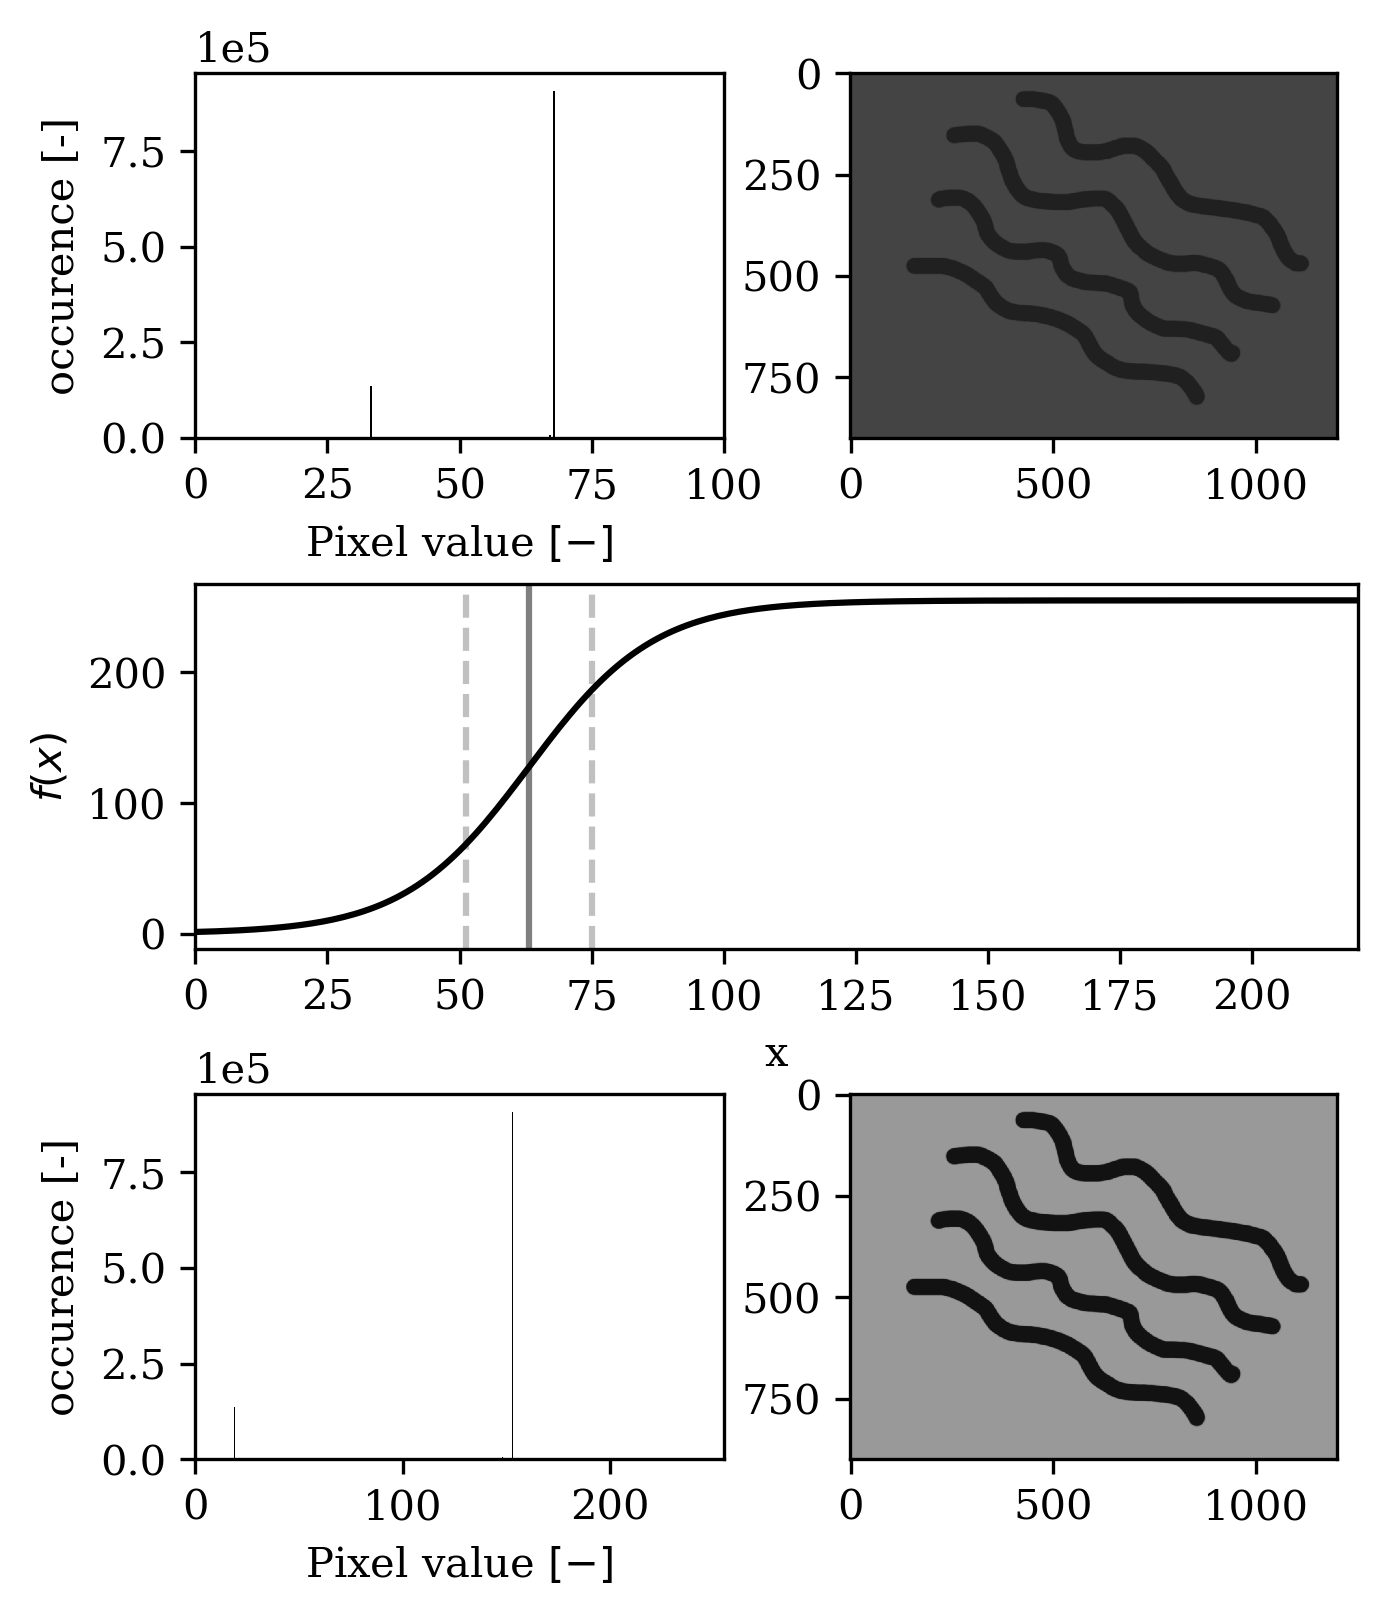
\includegraphics[width=0.55\textwidth,keepaspectratio]{afbeeldingen/sigmoid_explained.png}
    \caption{The example figure modified using a sigmoid function.}
    \label{fig:sigmoid}
\end{wrapfigure}

In figure \ref{fig:sigmoid} on the left, the low contrast example figure and its histogram are plotted in the top row. In the middle row a sigmoid function has been plotted, as well as the median value and the standard deviation of the histogram above denoted by respectively the grey solid and dashed line. The bottom row consists of the histogram of the example image and the image acted on by the sigmoid function. In this example we used a sigmoid function $f'(x)=f(x) \cdot 255$ since we want to map our input values on a domain $[0,255]$ not $[0,1]$, $\alpha$ is the median of the top histogram and $\beta$ its standard deviation.\\
As can be seen in the figure the peaks of the most common values of the intensity have been spread further apart thus resulting in a higher contrast image.\\


% FOURIER FILTERING

Rank filters are a type of linear filters that make use of the local gray scale pixel values. This type of first make a gray scale histogram of the pixels in the neighbourhood to applying local filters for smoothing, sharpening, noise reduction etc. (\cite{rank}).  
For this experiment, the bilateral mean filter, $BILAT$, the local contrast enhancement filter, $CONT$, and the local morphological contrast enhancement filter, $MORPH$, are implemented on the image of the fungus using the python Scikit-image package.\\
$BILAT$ makes the gray-level of pixels in a local neighbourhood similar to the central ones. It should therefore help to reduce noise. $CONT$ improves contrast for every local neighbourhood. $MORPH$ replaces a pixel values for either the local maximum or the local minimum. (\cite{rank}) \\
The image that is being used for this experiment is zoomed-in in order to see noise and fine details. A radius of $r_{local} = 20$ is used for $BILAT$, and for the other filters, a radius of $r_{local} = 5$ pixels is used for the local pixel neighbourhood. To explore how the image can be improved best, the filters are used in different combinations and compared.
\clearpage

\begin{comment}
The Experimentele opstelling or Experimentele  methode (Experimental  set  up  or  Experimental method) chapter describes the experimental setup and the experimental methods used in sufficient detail such that a reader can judge the soundness and, in principle, may verify the conclusions of your research. Also,  this  chapter  should  be  informative  for  a  reader  who  wants  to  perform  similar  research.  Preferably  use clear sketches of the setup, rather than photographs. In this chapter you also describe the accuracywith which direct observables have been measured, and the accuracy of the important deduced quantities. Detailed accuracy calculations should be put in an Appendix
\end{comment}
